\kapitel{Code Metrics}
\addcontentsline{toc}{part}{Code Metrics}
\thispagestyle{plain}
\renewcommand\section{\stdsection}

\sectionroman{Test Overview}
This overview shows that all tests have been passed and that the duration of the tests is quite short so that the tests can be ran regularly.
\begin{figure}[H]
    \centering
    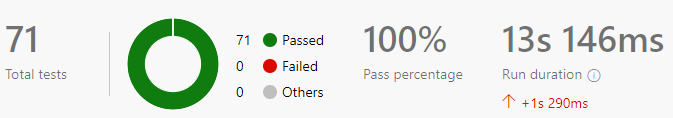
\includegraphics[width=1\linewidth]{assets/metrics/test_passing.png}
    \caption{Test Overview}
\end{figure}


\sectionroman{Test Scores}
As predicted at the beginning of the implementation there will not be a 100\% test coverage because several functions depend on system internal functions and outputs. Although, we could reach almost 50\% test coverage within 71 tests.
\begin{figure}[H]
    \centering
    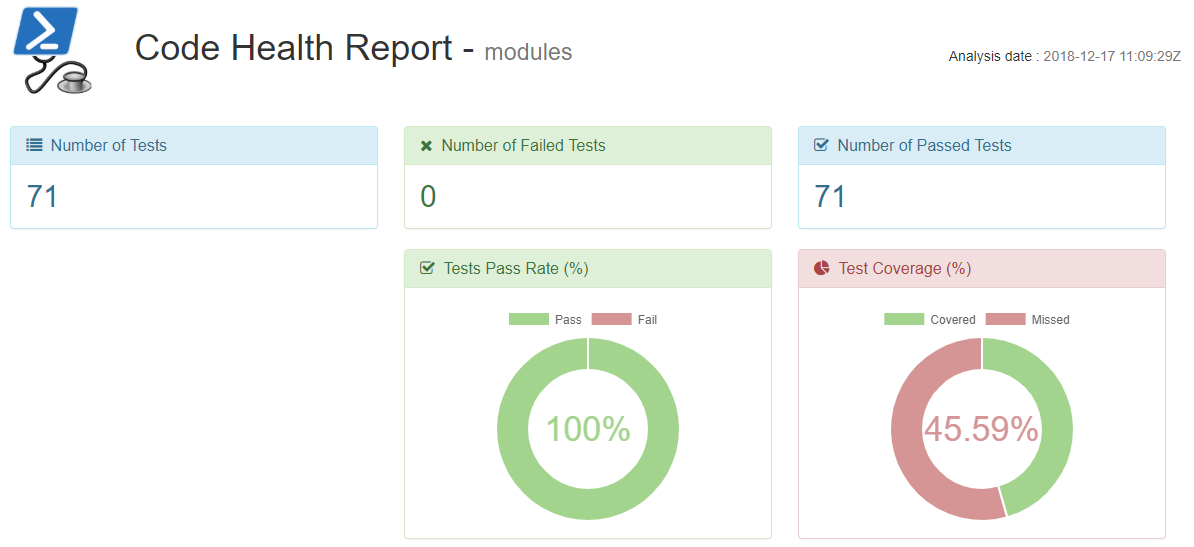
\includegraphics[width=1\linewidth]{assets/metrics/tests.png}
    \caption{Test Scores}
\end{figure}

\sectionroman{Maintainability}
The maintainability of the code is quite good, because the average functional length of code is well readable with almost 15 lines. The highest nesting depth is not quite as good, although PSCodeHealth marks it as ok. This nesting depth occurs in the functions \lstinline|GetAuditSettingValues| and \lstinline|ToolCanBeDetected|, but could not be solved otherwise.  
\begin{figure}[H]
    \centering
    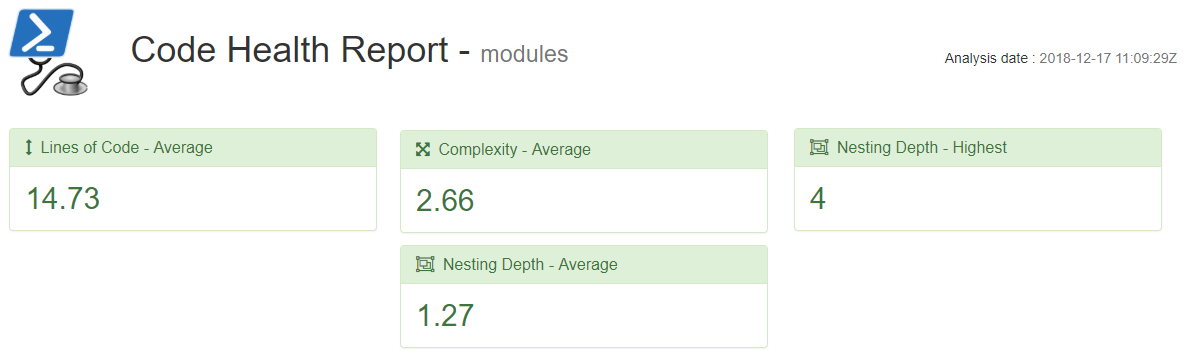
\includegraphics[width=1\linewidth]{assets/metrics/maintainability.png}
    \caption{Maintainability Scores}
\end{figure}